\documentclass[12pt,oneside]{article} % Uma Coluna e lingua portuguesa
%\usepackage[T1]{fontenc}        % Permite digitar os acentos de forma normal
\usepackage[utf8]{inputenc}
%\usepackage[english]{babel}
% \usepackage[portuges,brazil]{babel}
\usepackage[brazilian]{babel}

%\usepackage[latin1]{inputenc}
\usepackage[dvips]{graphicx}    % Permite Gráficos
%\usepackage{times}    % Fonte Times
\usepackage{fancyhdr}
\usepackage{array}
\usepackage{multicol}
\usepackage[colorlinks=true,linkcolor=blue,urlcolor=blue]{hyperref}
\usepackage{nomencl}    % glossario
\usepackage{amssymb}
\usepackage{amsmath}
\usepackage[compact]{titlesec}
\usepackage{wrapfig}
\usepackage{color}
\usepackage{csquotes}

%=======================================================================

% Hifenização das palavras desconhecidas pelo LaTeX
%\hyphenation{}
\paperheight    297mm
\paperwidth     210mm
\voffset         -15mm
\headheight      15pt %% tamanho de letra
\headsep         5mm  %% para o início do texto
\oddsidemargin  -3.0mm
\evensidemargin -3.0mm
\textwidth      167.0mm
\topmargin      005.0mm
\textheight     240.0mm
\footskip       10.0mm

\title{PPCI 2024 - Maratona de Programação}

\author{Maratona de Programação}
\date{19 de outubro de 2024}
\usepackage{indentfirst}
\usepackage{subfig}

\parindent=0pt
\setlength{\parskip}{7pt plus 1pt minus 2pt}
\titlespacing{\section}{0pt}{*0}{*0}
\titlespacing{\subsection}{0pt}{*0}{*0}
\titlespacing{\subsubsection}{0pt}{*0}{*0}

\begin{document}

\begin{center}
\textbf{\Huge PPCI 2024 - Maratona de Programação} \\
\vspace{0.2cm}
\textit{19 de outubro de 2024} \\
\vspace{1.0cm}
%\textbf{Sevidor BOCA:} \\
%\texttt{\large http://maratona.c3sl.ufpr.br/boca/} \\
%\vspace{1.0cm}
\begin{figure}[h!]
    \centering
    
\includegraphics[scale=0.72]{capa.png}
\end{figure}

\begin{figure}[h!]
    \centering
    
\includegraphics[scale=0.20]{logo-PPCI.png}
\end{figure}
\vspace{1.0cm}
%\textbf{Organizadores:}\\
%{\small Flávio Zavan} \\
%{\small Ricardo Oliveira} \\
\vspace{1.0cm}
\end{center}

\clearpage

\pagestyle{fancy}
\renewcommand{\footrulewidth}{0.7pt}
\renewcommand{\headrulewidth}{0.7pt}
\lhead{PPCI 2024}
\chead{Maratonas de Programação}
\rhead{19 de outubro de 2024}
\cfoot{\thepage}

\newpage

% Espaco para o create-zips.sh nao achar
  \section*{Instruções Importantes}

\begin{itemize}

    \item Use a opção \textbf{Runs} para enviar suas soluções. Os problemas podem resolvidos em qualquer ordem e
    linguagem (dentre C, C++ e Python, independentemente do problema);

    \item Suas soluções serão testadas com várias entradas,
    além das dadas como exemplo. Por isso, sua solução pode não ser
    aceita mesmo se funcionar para os exemplos dados. Certifique-se que ela
    funciona para todas as entradas possíveis;

    \item A saída gerada deve ser \textit{exatamente} conforme
    especificada. Em particular, \textbf{não} imprima instruções (``digite um
            número'', ``a resposta é'', etc);

    \item É garantido que todas as entradas usadas para teste estarão de acordo
    com o enunciado, não sendo necessário testar se são válidas;

    \item Ao enviar uma solução, o sistema irá responder uma das
    seguintes respostas:
    \begin{itemize}
        \item \verb|Not answered yet|: a solução está sendo corrigida.
        Aguarde um pouco e atualize a página;
        \item \verb|YES|: solução aceita. Parabéns!
        \item \verb|Wrong Answer|: a saída impressa pelo seu programa não é a
        saída correta esperada, para alguma entrada de teste;
        \item \verb|Presentation Error|: a saída impressa está correta, exceto
        por espaços em branco e/ou quebras-de-linha faltando/sobrando;
        \item \verb|Time Limit Exceeded|: o tempo de execução do seu programa
        ultrapassou o tempo limite estipulado para o problema (ver tabela
        abaixo). O tempo de execução da sua solução precisa ser menor;
        \item \verb|Runtime Error|: seu programa gerou algum erro em tempo de
        execução (``crashou'');
        \item \verb|Compile Error|: seu programa não compila.
    \end{itemize}

    \item Todas as linhas, tanto na entrada quanto na saída, terminam com o
    caractere de fim-de-linha ($\backslash n$), mesmo quando houver apenas uma única
    linha na entrada e/ou saída;

    \newpage
    \item Sua solução deve processar cada arquivo de entrada no tempo máximo
    estipulado para cada problema, dado pela seguinte tabela:

    \begin{table}[h]
    \centering
    \begin{tabular}{|c|c||c|}
    \hline
    \textbf{Problema} & \textbf{Nome} & \textbf{Tempo Limite (segundos)} \\
    \hline
    A & Arremesso de Triângulo & 1 \\
    B & Bloons & 1 \\
    C & Cofre Break & 1 \\
    D & Double Casting & 1 \\
    E & Estresse & 1 \\ % mudar talvez
    F & Futebol & 1 \\
    G & Graffiti & 1 \\
    H & Herança & 1 \\ % mudar talvez
    I & Ímpar e Impares & 1 \\
    J & Joias do Tesouro & 1 \\
    K & Kleber e a Convenção & 1 \\
    L & Lâmpada Maldita & 1 \\
    \hline
    \end{tabular}
    \end{table}

\end{itemize}

\newpage
\section*{A: Arremesso de Triângulo} %tle=1
\vspace{-0.52cm}
\noindent \begin{verbatim}Arquivo: arremesso.[c|cpp|py]\end{verbatim}
As Olimpíadas de Verão Nlogônia 2024 estão sendo um sucesso! Inúmeros atletas
estão em busca da tão sonhada medalha de ouro em diversos esportes.

Um dos esportes disputados é o \textit{arremesso de trinângulo}. Este esporte é
jogado em um campo que pode ser representado em um plano cartesiano. O campo
contém $N$ semicircunferências. Seus raios são $r_1$, $r_2$, ..., $r_N$ em ordem
crescente, todas são centradas na origem, e cada semicircunferência tem seu
\textit{valor} associado.

A figura abaixo exemplifica um campo com $N=3$
semicircunferências, de raios 2, 3 e 5, e valores 2, 1 e 4, respectivamente:

\begin{center}
    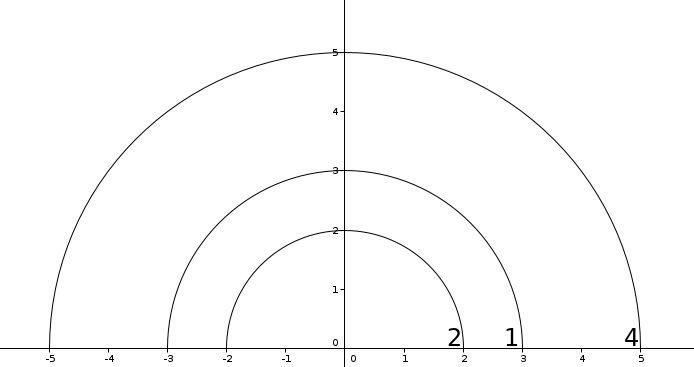
\includegraphics[scale=0.4]{arremesso/campo.png}
\end{center}

Em uma jogada, um atleta arremessa um ponto em uma posição $P$. Em seguida, é
traçado um triângulo cujos vértices são os pontos $P$, $(X_L, 0)$ e $(X_R, 0)$
(os valores de $X_L$ e $X_R$ são definidos pelos juizes). Como exemplo,
considere que um atleta arremessou um ponto na posição $P=(4,5)$, que $X_L = -4$
e $X_R = 1$. A figura abaixo mostra o triângulo traçado:

\begin{center}
    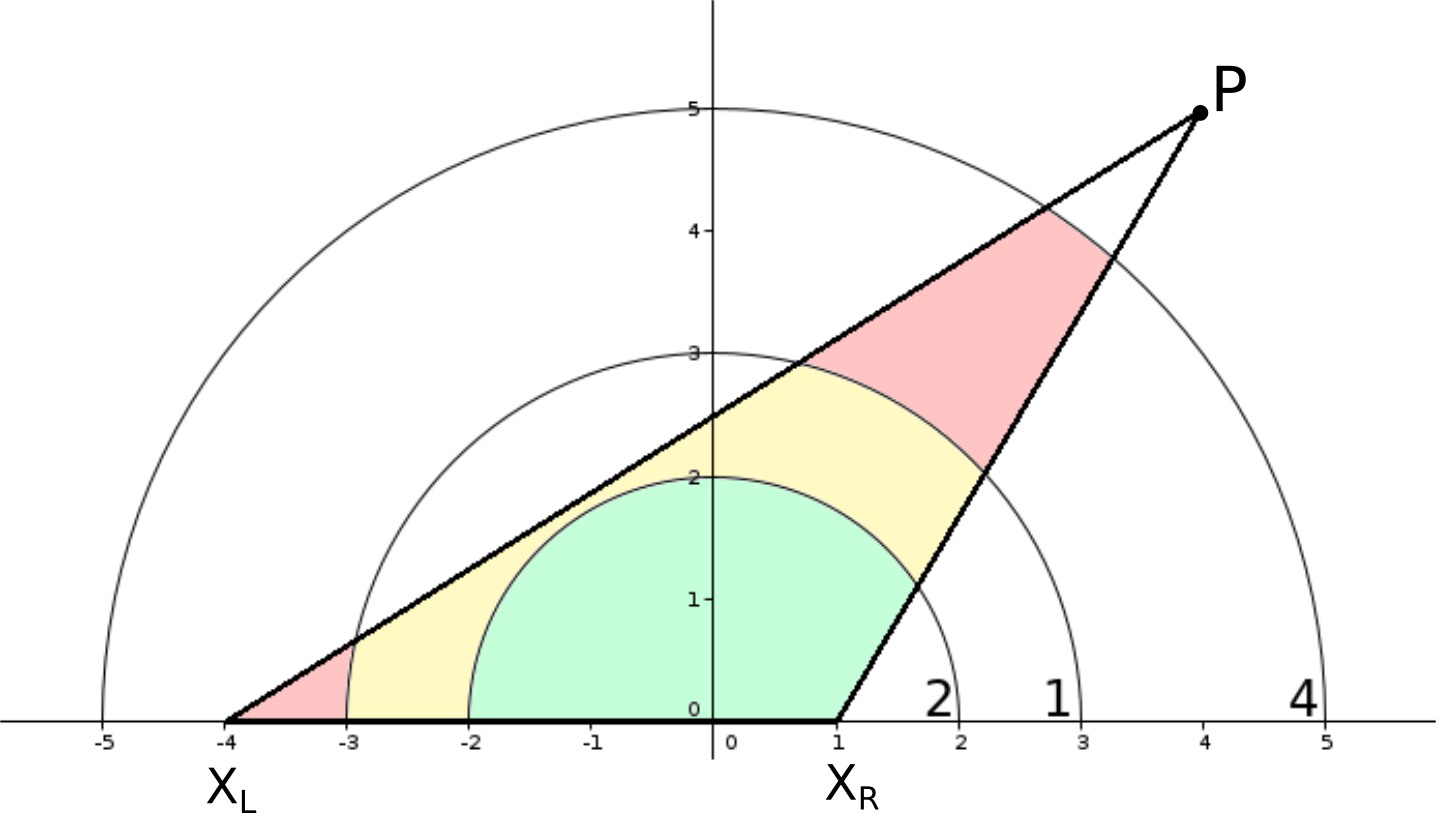
\includegraphics[scale=0.4]{arremesso/score.png}
\end{center}

A \textit{região de pontuação} de uma semicircunferência é a área do seu
semicírculo (no caso da primeira semicircunferência) ou a área entre uma
semicircunferência e a próxima semicircunferência (no caso das demais).

A \textit{pontuação} feita em uma semicircunferência é dada pelo produto entre
seu valor e a área de intersecção entre o triângulo e sua região de pontuação.
A \textit{pontuação total} da jogada é dada pela soma da pontuação feita em
todas as semicircunferências.

No exemplo dado, a pontuação total da jogada será, aproximadamente,
2 $\times$ 5.662733 (a área em verde na figura)
+ 1 $\times$ 3.579953 (a área em amarelo na figura)
+ 4 $\times$ 2.774575 (a área em vermelho na figura)
$\approx$ 26.003719.

Dada a descrição do campo e da jogada, determine sua pontuação total.

\subsection*{Entrada}

A primeira linha contém um inteiro $N$ ($1 \leq N \leq 100$), o número de
semicircunferencias no campo. A próxima linha contém $N$ inteiros $r_i$
$(1 \leq r_i \leq 100)$, os raios das semicircunferências, em ordem crescente.
A próxima linha contém $N$ inteiros $v_i$
$(0 \leq v_i \leq 10$), os valores de cada semicircunferência, na ordem em que são
dados na entrada.
A próxima linha contém dois inteiros $X_L$ e $X_R$
$(-100 \leq X_L \leq 0 \leq X_R \leq 100)$ indicando as coordenadas definidas pelos juizes. A última linha contém dois inteiros
$X_P$ e $Y_P$ ($-100 \leq X_P \leq 100$, $0 \leq Y_P \leq 100$) indicando a
coordenada do ponto arremessado.

Note que tanto os pontos $(X_L,0)$ e $(X_R,0)$ quanto o ponto
$P$ podem ou não estar dentro de algum semi-circulo.

\subsection*{Saída}

Imprima uma única linha contendo a pontuação total da jogada, arredondada com
exatamente duas casas decimais.

%----- Exemplo 1 -----%
\begin{table}[!h]
\centering
\begin{tabular}{|l|l|}
\hline
\begin{minipage}[t]{3in}
\textbf{Exemplo de entrada}
\begin{verbatim}
3
2 3 5
2 1 4
-4 1
4 5
\end{verbatim}
\vspace{1mm}
\end{minipage}
&
\begin{minipage}[t]{3in}
\textbf{Exemplo de saída}
\begin{verbatim}
26.00
\end{verbatim}
\vspace{1mm}
\end{minipage} \\
\hline
\end{tabular}
\end{table}

%----- Exemplo 2 -----%
\begin{table}[!h]
\centering
\begin{tabular}{|l|l|}
\hline
\begin{minipage}[t]{3in}
\textbf{Exemplo de entrada}
\begin{verbatim}
4
1 5 7 8
2 1 0 1
-10 10
0 10
\end{verbatim}
\vspace{1mm}
\end{minipage}
&
\begin{minipage}[t]{3in}
\textbf{Exemplo de saída}
\begin{verbatim}
55.02
\end{verbatim}
\vspace{1mm}
\end{minipage} \\
\hline
\end{tabular}
\end{table}


\newpage
\section*{B: Bloons} %tle=1
\vspace{-0.52cm}
\noindent \begin{verbatim}Arquivo: bloons.[c|cpp|py]\end{verbatim}
No jogo \textbf{Bloons Tower Defense}, existem macacos que defendem o território deles, que é constantemente atacado por uma sequência de balões com diferentes camadas de resistência. Cada macaco pode arremessar dardos que dão dano e destroem um número específico de camadas de um balão. Cada balão, por sua vez, tem um número de camadas a serem destruídas. Um balão só é totalmente destruído quando o último dardo que o acertar der dano \textbf{exatamente} igual à quantidade de camadas restantes do balão.

Dada uma sequência de $N$ balões, onde cada balão tem $h_i$ camadas (ou seja, o balão $i$ tem resistência $h_i$), temos disponíveis $K$ tipos de macacos, onde o macaco do tipo $j$ pode arremessar um dardo que destrói exatamente $d_j$ camadas de um balão.

Você deve determinar o número mínimo de dardos necessários para destruir completamente todos os balões da sequência. Se não for possível destruir todos os balões, retorne -1. E lembrando que um balão é totalmente destruído somente se os dano causado nele é \textbf{exatamente} o número de camadas dele. E ressaltando também que o mesmo macaco pode arremessar dardos quantas vezes quiser em qualquer balão.

\subsection*{Entrada}
    A primeira linha contém dois inteiros $N$ $(1 \leq N \leq 1000)$ e $K$ $(1 \leq K \leq 100)$, representando o número de balões e o número de macacos, respectivamente.

    A segunda linha contém $N$ inteiros, onde o $i$-ésimo inteiro representa $h_i$ $(1 \leq h_i \leq 1000)$, o número de camadas de resistência do $i$-ésimo balão.

    A terceira linha contém $K$ inteiros, onde o $j$-ésimo inteiro representa $d_j$ $(1 \leq d_j \leq 1000)$, o número de camadas que o dardo arremessado pelo $j$-ésimo macaco consegue destruir.

\subsection*{Saída}
Imprima o número mínimo de dardos necessários para destruir todos os balões. Se não for possível destruir todos os balões, imprima -1.

%----- Exemplo 1 -----%
\newpage
\begin{table}[!h]
\centering
\begin{tabular}{|l|l|}
\hline
\begin{minipage}[t]{3in}
\textbf{Exemplo de entrada}
\begin{verbatim}
4 3
5 10 6 8
2 3 5
\end{verbatim}
\vspace{1mm}
\end{minipage}
&
\begin{minipage}[t]{3in}
\textbf{Exemplo de saída}
\begin{verbatim}
7
\end{verbatim}
\vspace{1mm}
\end{minipage} \\
\hline
\end{tabular}
\end{table}

%----- Exemplo 2 -----%
\begin{table}[!h]
\centering
\begin{tabular}{|l|l|}
\hline
\begin{minipage}[t]{3in}
\textbf{Exemplo de entrada}
\begin{verbatim}
2 2
7 11
2 5
\end{verbatim}
\vspace{1mm}
\end{minipage}
&
\begin{minipage}[t]{3in}
\textbf{Exemplo de saída}
\begin{verbatim}
6
\end{verbatim}
\vspace{1mm}
\end{minipage} \\
\hline
\end{tabular}
\end{table}


%----- Exemplo 3 -----%
\begin{table}[!h]
\centering
\begin{tabular}{|l|l|}
\hline
\begin{minipage}[t]{3in}
\textbf{Exemplo de entrada}
\begin{verbatim}
2 2
7 8
3 5
\end{verbatim}
\vspace{1mm}
\end{minipage}
&
\begin{minipage}[t]{3in}
\textbf{Exemplo de saída}
\begin{verbatim}
-1
\end{verbatim}
\vspace{1mm}
\end{minipage} \\
\hline
\end{tabular}
\end{table}


% Quero a cor vermelha nesse problema!
\newpage
\section*{C: Cofre Break} %tle=1
\vspace{-0.52cm}
\noindent \begin{verbatim}Arquivo: cofre-break.[c|cpp|py]\end{verbatim}
Carlinhos é um grande colecionador de balões e, para proteger sua preciosa coleção, decidiu trancá-la em um cofre com uma senha \textit{s}, composta por \textit{n} números inteiros.
Porém, a memória de Carlinhos não é a das melhores, então ele decidiu escrever a senha em um papel e guardá-la em um lugar seguro.
No entanto, para garantir que ninguém descubra a senha, Carlinhos resolveu anotá-la de maneira camuflada, seguindo uma regra especial:

\begin{itemize}
    \item A maior sequência de números distintos, ou seja, a maior sequência contínua de números onde nenhum número aparece mais de uma vez, foi invertida.
    \item Caso haja mais de uma sequência de maior tamanho, apenas a primeira, da esquerda para a direita, será invertida.
    \item O restante dos números foi mantido na mesma ordem original.
\end{itemize}

Agora, anos depois, Carlinhos quer pegar seu balão vermelho favorito, mas sua memória falhou novamente. 
Ele não lembra qual sequência havia sido invertida, e tudo o que tem é a versão modificada da senha que ele escreveu no papel.

A sua tarefa é ajudar Carlinhos a pegar o seu balão favorito, descobrindo a senha correta do cofre.

\subsection*{Entrada}

A primeira linha contém um inteiro $n$ ($1 \leq n \leq 10^5$), que representa a quantidade de números da senha.

A segunda linha contém $n$ inteiros $s_i$ ($0 \leq s_i \leq 10^9$), que representam os dígitos da senha como foram escritos no papel.

\subsection*{Saída}

Imprima a senha correta para o cofre, separando os números por espaços. Não imprima o espaço após o último número.

\newpage
%----- Exemplo 1 -----%
\begin{table}[!h]
\centering
\begin{tabular}{|l|l|}
\hline
\begin{minipage}[t]{3in}
\textbf{Exemplo de entrada}
\begin{verbatim}
7
1 1 2 3 4 5 5
\end{verbatim}
\vspace{1mm}
\end{minipage}
&
\begin{minipage}[t]{3in}
\textbf{Exemplo de saída}
\begin{verbatim}
1 5 4 3 2 1 5
\end{verbatim}
\vspace{1mm}
\end{minipage} \\
\hline
\end{tabular}
\end{table}

%----- Exemplo 2 -----%
\begin{table}[!h]
\centering
\begin{tabular}{|l|l|}
\hline
\begin{minipage}[t]{3in}
\textbf{Exemplo de entrada}
\begin{verbatim}
9
1 2 1 3 4 7 3 5 7
\end{verbatim}
\vspace{1mm}
\end{minipage}
&
\begin{minipage}[t]{3in}
\textbf{Exemplo de saída}
\begin{verbatim}
1 7 4 3 1 2 3 5 7
\end{verbatim}
\vspace{1mm}
\end{minipage} \\
\hline
\end{tabular}
\end{table}

%----- Exemplo 3 -----%
\begin{table}[!h]
\centering
\begin{tabular}{|l|l|}
\hline
\begin{minipage}[t]{3in}
\textbf{Exemplo de entrada}
\begin{verbatim}
6
42 42 43 43 44 44
\end{verbatim}
\vspace{1mm}
\end{minipage}
&
\begin{minipage}[t]{3in}
\textbf{Exemplo de saída}
\begin{verbatim}
42 43 42 43 44 44
\end{verbatim}
\vspace{1mm}
\end{minipage} \\
\hline
\end{tabular}
\end{table}


% Quero a cor azul nesse problema!
\newpage
\section*{D: Double Casting} %tle=1
\vspace{-0.52cm}
\noindent \begin{verbatim}Arquivo: double_casting.[c|cpp|py]\end{verbatim}
Mikio descobriu uma nova mecânica no seu jogo favorito \textit{Lost in Time (LIT)}, o \textbf{double casting}, no qual ele pode usar duas magias ao mesmo tempo caso o dano delas seja igual.

Em \textit{LIT} você deve comprar suas magias utilizando as LIT coins, o custo da magia é igual ao valor do dano dela em LIT coins e cada magia é de uso único. A loja de magias possui $N$ magias.

Você pode comprar apenas um único intervalo $(1\leq i \leq j \leq N)$ de magias, que custará o valor da soma de todas as magias dentro deste intevalo, ou seja \textbf{soma}$[i; j]$ = ($a_i + a_{i+1}+ a_{i+2}+ ...+ a_j$).

Mikio possui apenas $K$ LIT coins e deseja realizar o máximo de \textbf{double casting's} possíveis.


\subsection*{Entrada}

A primeira linha contém dois inteiro $N$ ($1 \leq N \leq 2\cdot 10^5$) e $K$ $(1 \leq k \leq 10^9$), o número de magias da loja e o total de LIT coins que Mikio possui, respectivamente.

A próxima linha contém $N$ inteiros $a_i$ $(1 \leq a_i \leq 10^9$), o custo das magias da loja.

\subsection*{Saída}

Imprima o maior número de \textbf{double casting's} que Mikio pode realizar.

%----- Exemplo 1 -----%
\begin{table}[!h]
\centering
\begin{tabular}{|l|l|}
\hline
\begin{minipage}[t]{3in}
\textbf{Exemplo de entrada}
\begin{verbatim}
5 20
1 3 2 1 3
\end{verbatim}
\vspace{1mm}
\end{minipage}
&
\begin{minipage}[t]{3in}
\textbf{Exemplo de saída}
\begin{verbatim}
2
\end{verbatim}
\vspace{1mm}
\end{minipage} \\
\hline
\end{tabular}
\end{table}

%----- Exemplo 2 -----%
\begin{table}[!h]
\centering
\begin{tabular}{|l|l|}
\hline
\begin{minipage}[t]{3in}
\textbf{Exemplo de entrada}
\begin{verbatim}
7 26
2 20 2 3 10 10 3
\end{verbatim}
\vspace{1mm}
\end{minipage}
&
\begin{minipage}[t]{3in}
\textbf{Exemplo de saída}
\begin{verbatim}
2
\end{verbatim}
\vspace{1mm}
\end{minipage} \\
\hline
\end{tabular}
\end{table}

%----- Exemplo 3 -----%
\begin{table}[!h]
\centering
\begin{tabular}{|l|l|}
\hline
\begin{minipage}[t]{3in}
\textbf{Exemplo de entrada}
\begin{verbatim}
4 1000
1 100000 1 13
\end{verbatim}
\vspace{1mm}
\end{minipage}
&
\begin{minipage}[t]{3in}
\textbf{Exemplo de saída}
\begin{verbatim}
0
\end{verbatim}
\vspace{1mm}
\end{minipage} \\
\hline
\end{tabular}
\end{table}


\newpage
\section*{E: Estresse} %tle=1
\vspace{-0.52cm}
\noindent \begin{verbatim}Arquivo: estresse.[c|cpp|py]\end{verbatim}
Às vezes, é preciso ter aquela conversa difícil e dizer o que é necessário. É ou não é?

Yara e sua colega Karen compartilham o mesmo apartamento. A papagaia da Karen, Lori, fica o dia todo presa na gaiola, sem ninguém para conversar, pois Karen estuda o dia inteiro e só chega de noite para dar atenção à coitada. Yara tem dó da passarinha, e precisa mostrar para Karen como a passarinha se sente abandonada e que é preciso tomar uma providência.

Yara é estudante de biologia, e por observação chegou à hipótese de que papagaios falam muito quando estressados, e às vezes também podem falar ao contrário, de trás para frente. Então, ela gravou a papagaia ao longo de um dia e obteve uma string $S$, que contém letras correspondentes a sons, os quais podem ter sido falas da Lori ou ruídos de fundo. A bichana sempre fala a mesma palavra $P$, podendo ser de frente para trás ou de trás para frente. 

É preciso que você conte em quantos momentos, ao longo da gravação, houve um som que possa ter sido a Lori falando. Dessa forma, Yara poderá estudar o caso, e quem sabe mostrar para Karen como o comportamento da Lori é consequência da tristeza e estresse de estar sozinha e sem interação o dia inteiro.


\subsection*{Entrada}
A primeira linha contém uma string $S$, de tamanho $|S|$ ($1\leq |S|\leq 2\cdot 10^5$).

A segunda linha contém uma string $P$, de tamanho $|P|$ ($1\leq |P|\leq 2\cdot 10^5$).

Ambas strings são formadas por caracteres minúsculos do alfabeto inglês (i.e. de \texttt{`a'} a \texttt{`z'}).


\subsection*{Saída}
Imprima a quantidade de momentos distintos da gravação em que houve um som que possa ser a papagaia falando.


%----- Exemplo 1 -----%
\newpage
\begin{table}[!h]
\centering
\begin{tabular}{|l|l|}
\hline
\begin{minipage}[t]{3in}
\textbf{Exemplo de entrada}
\begin{verbatim}
zzzgrrauauzzz
uauarrg
\end{verbatim}
\vspace{1mm}
\end{minipage}
&
\begin{minipage}[t]{3in}
\textbf{Exemplo de saída}
\begin{verbatim}
1
\end{verbatim}
\vspace{1mm}
\end{minipage} \\
\hline
\end{tabular}
\end{table}

%----- Exemplo 2 -----%
\begin{table}[!h]
\centering
\begin{tabular}{|l|l|}
\hline
\begin{minipage}[t]{3in}
\textbf{Exemplo de entrada}
\begin{verbatim}
orolorolouolorolol
loro
\end{verbatim}
\vspace{1mm}
\end{minipage}
&
\begin{minipage}[t]{3in}
\textbf{Exemplo de saída}
\begin{verbatim}
5
\end{verbatim}
\vspace{1mm}
\end{minipage} \\
\hline
\end{tabular}
\end{table}


%----- Exemplo 3 -----%
\begin{table}[!h]
\centering
\begin{tabular}{|l|l|}
\hline
\begin{minipage}[t]{3in}
\textbf{Exemplo de entrada}
\begin{verbatim}
arararara
arara
\end{verbatim}
\vspace{1mm}
\end{minipage}
&
\begin{minipage}[t]{3in}
\textbf{Exemplo de saída}
\begin{verbatim}
3
\end{verbatim}
\vspace{1mm}
\end{minipage} \\
\hline
\end{tabular}
\end{table}


\newpage
\section*{F: Futebol} %tle=1
\vspace{-0.52cm}
\noindent \begin{verbatim}Arquivo: futebol.[c|cpp|py]\end{verbatim}
O futebol é o esporte mais popular do mundo, com entusiastas espalhados globalmente. Rafael, além de ser um grande fã do esporte, também é analista de desempenho de um clube de futebol profissional chamado Universitários FC.

O técnico do time solicitou que Rafael desenvolvesse um programa para ajudar o time a melhorar suas chances de marcar gols. Contudo, Rafael não é especialista em programação, e por isso ele decidiu pedir a sua ajuda para resolver este problema.

A sua tarefa é criar um programa que analise se é possível que o Universitários FC troque passes de maneira eficiente, de modo que a bola saia dos pés do goleiro e chegue até o centroavante, o jogador responsável por finalizar as jogadas.

A entrada do programa consiste nas possíveis opções de passes entre os jogadores. Cada passe indica que a bola pode ser passada de um jogador X para um jogador Y (e vice-versa). Note que as opções de passes podem ser limitadas, o programa deve encontrar o tamanho do menor caminho possível que a bola fará entre os jogadores. Em outras palavras, o programa deve mostrar a quantidade mínima de jogadores que participarão na sequência de passes, de forma que o número total de jogadores envolvidos seja o menor possível.

\subsection*{Entrada}

A primeira linha contém um número inteiro $N$ ($1 \leq N \leq 55$), representando o número de passes possíveis.

As próximas $N$ linhas descrevem as opções de passe, onde a bola pode ser passada do jogador X para o jogador Y e vice-versa. Os jogadores são numerados de 1 a 11, sendo que o jogador 1 é o goleiro e o jogador 9 é o centroavante.

\subsection*{Saída}

Imprima a quantidade mínima de jogadores que participarão da troca de passes, incluindo o goleiro (jogador 1) e o centroavante (jogador 9).

Caso não seja possível completar a sequência de passes até o centroavante, imprima $-1$.

%----- Exemplo 1 -----%
\begin{table}[!h]
\centering
\begin{tabular}{|l|l|}
\hline
\begin{minipage}[t]{3in}
\textbf{Exemplo de entrada}
\begin{verbatim}
11
1 3
1 4
3 2
4 6
3 5
5 10
5 8
10 8
2 7
10 11
11 9
\end{verbatim}
\vspace{1mm}
\end{minipage}
&
\begin{minipage}[t]{3in}
\textbf{Exemplo de saída}
\begin{verbatim}
6
\end{verbatim}
\vspace{1mm}
\end{minipage} \\
\hline
\end{tabular}
\end{table}

%----- Exemplo 2 -----%
\begin{table}[!h]
\centering
\begin{tabular}{|l|l|}
\hline
\begin{minipage}[t]{3in}
\textbf{Exemplo de entrada}
\begin{verbatim}
9
1 3
1 4
3 2
4 6
4 5
5 10
5 8
11 9
9 7
\end{verbatim}
\vspace{1mm}
\end{minipage}
&
\begin{minipage}[t]{3in}
\textbf{Exemplo de saída}
\begin{verbatim}
-1
\end{verbatim}
\vspace{1mm}
\end{minipage} \\
\hline
\end{tabular}
\end{table}

%----- Exemplo 3 -----%
\begin{table}[!h]
\centering
\begin{tabular}{|l|l|}
\hline
\begin{minipage}[t]{3in}
\textbf{Exemplo de entrada}
\begin{verbatim}
13
1 3
1 4
3 2
4 6
3 5
4 5
5 10
5 8
10 11
8 7
1 9
11 9
7 9
\end{verbatim}
\vspace{1mm}
\end{minipage}
&
\begin{minipage}[t]{3in}
\textbf{Exemplo de saída}
\begin{verbatim}
2
\end{verbatim}
\vspace{1mm}
\end{minipage} \\
\hline
\end{tabular}
\end{table}

\newpage

\section*{G: Graffiti} %tle=1
\vspace{-0.52cm}
\noindent \begin{verbatim}Arquivo: graffiti.[c|cpp|py]\end{verbatim}
Guilherme e Gabriela são dois irmãos apaixonados por arte. Desde pequenos, sempre competiram para ver quem conseguia criar o melhor desenho. Desta vez, eles decidiram transformar o muro de casa em uma obra de arte colorida, utilizando graffiti. Cada um tem uma cor favorita: Gabriela gosta de laranja, enquanto Guilherme prefere o roxo. No entanto, essa simples discordância transformou a atividade em uma competição. Como em qualquer disputa entre irmãos, o objetivo não é apenas grafitar, mas ver quem consegue cobrir a maior área do muro com sua cor favorita.

O muro possui uma altura fixa de 1 metro e inicialmente está em branco. Gabriela e Guilherme se revezam para grafitar. Como Gabriela é mais velha, ela sempre começa. A cada turno, eles escolhem uma posição e uma distância horizontal no muro, e toda a área dentro dessa distância é grafitada.

Como ambos são extremamente competitivos, eles podem grafitar por cima das cores já preenchidas pelo outro, e a cor mais recente prevalece em cada posição.

\subsection*{Entrada}

A primeira linha contém dois inteiros \textit{n} e \textit{m} ($1 \leq \textit{n} \leq 10^5, 1 \leq \textit{m} \leq 10^5$), representando o comprimento do muro em metros e o número de turnos, respectivamente.

As próximas \textit{m} linhas descrevem as ações dos irmãos em cada turno.

Cada uma dessas linhas contém dois inteiros \textit{$p_i$} e \textit{$d_i$} ($0 \leq \textit{$p_i$} < \textit{n}, 1 \leq \textit{$d_i$} \leq n - p_i$), onde \textit{$p_i$} é a posição inicial,  começando de 0, e \textit{d} é a distância grafitada a partir dessa posição.

\subsection*{Saída}

Imprima o nome do irmão que grafitou a maior área da parede. Se ambos grafitaram a mesma área, imprima "Empate".

\newpage

%----- Exemplo 1 -----%
\begin{table}[!h]
\centering
\begin{tabular}{|l|l|}
\hline
\begin{minipage}[t]{3in}
\textbf{Exemplo de entrada}
\begin{verbatim}
8 4
0 4
4 4
0 8
3 3
\end{verbatim}
\vspace{1mm}
\end{minipage}
&
\begin{minipage}[t]{3in}
\textbf{Exemplo de saída}
\begin{verbatim}
Gabriela
\end{verbatim}
\vspace{1mm}
\end{minipage} \\
\hline
\end{tabular}
\end{table}

%----- Exemplo 2 -----%
\begin{table}[!h]
\centering
\begin{tabular}{|l|l|}
\hline
\begin{minipage}[t]{3in}
\textbf{Exemplo de entrada}
\begin{verbatim}
10 7
0 10
0 8
2 7
3 4
4 2
8 2
5 1
\end{verbatim}
\vspace{1mm}
\end{minipage}
&
\begin{minipage}[t]{3in}
\textbf{Exemplo de saída}
\begin{verbatim}
Guilherme
\end{verbatim}
\vspace{1mm}
\end{minipage} \\
\hline
\end{tabular}
\end{table}

%----- Exemplo 3 -----%
\begin{table}[!h]
\centering
\begin{tabular}{|l|l|}
\hline
\begin{minipage}[t]{3in}
\textbf{Exemplo de entrada}
\begin{verbatim}
12 8
0 1
1 11
5 6
7 3
2 2
0 5
0 8
2 3
\end{verbatim}
\vspace{1mm}
\end{minipage}
&
\begin{minipage}[t]{3in}
\textbf{Exemplo de saída}
\begin{verbatim}
Empate
\end{verbatim}
\vspace{1mm}
\end{minipage} \\
\hline
\end{tabular}
\end{table}


\newpage
\section*{H: Herança} %tle=1
\vspace{-0.52cm}
\noindent \begin{verbatim}Arquivo: heranca.[c|cpp|py]\end{verbatim}
Você acaba de receber uma notícia inesperada: seu tio-avô, morador de Nlogônia, faleceu e deixou uma herança especial para você. Porém, sabendo da sua paixão por problemas de lógica e desafios matemáticos, ele deixou um enigma como parte de sua herança.

Na casa dele, você encontra uma mochila mágica com um limite de peso $W$ que pode ser carregado dentro dela. Junto à mochila, há uma carta explicando que ela pode ser preenchida com uma série de itens valiosos, cada um com um peso e um valor específico. No entanto, você não precisa pegar os itens inteiros – pode escolher levar apenas uma fração de cada item, se assim desejar.

Seu desafio é simples: escrever um algoritmo que defina o valor máximo dos itens para o peso $w$ de sua mochila.

\subsection*{Entrada}

A primeira linha contém 2 inteiros $N$ ($1 \leq N \leq 10^5$) e $W$ ($1 \leq W \leq 10^3$) que indicam, respectivamente, o número de itens disponíveis e o peso máximo suportado pela mochila.

As próximas $N$ linhas contêm 2 inteiros $P$ ($1 \leq P \leq 10^6$) e $V$ ($1 \leq V \leq 10^8$) indicando o peso e o valor de cada item.

\subsection*{Saída}

Imprima um número com 2 casas após a vírgula, indicando o valor máximo.

Utilize números com precisão dupla.

%----- Exemplo 1 -----%
\begin{table}[!h]
\centering
\begin{tabular}{|l|l|}
\hline
\begin{minipage}[t]{3in}
\textbf{Exemplo de entrada}
\begin{verbatim}
3 50
10 60
20 100
30 120
\end{verbatim}
\vspace{1mm}
\end{minipage}
&
\begin{minipage}[t]{3in}
\textbf{Exemplo de saída}
\begin{verbatim}
240.00
\end{verbatim}
\vspace{1mm}
\end{minipage} \\
\hline
\end{tabular}
\end{table}

%----- Exemplo 2 -----%
\begin{table}[!h]
\centering
\begin{tabular}{|l|l|}
\hline
\begin{minipage}[t]{3in}
\textbf{Exemplo de entrada}
\begin{verbatim}
2 50
20 10
50 3
\end{verbatim}
\vspace{1mm}
\end{minipage}
&
\begin{minipage}[t]{3in}
\textbf{Exemplo de saída}
\begin{verbatim}
11.80
\end{verbatim}
\vspace{1mm}
\end{minipage} \\
\hline
\end{tabular}
\end{table}



\newpage
\section*{I: Ímpar e Impares} %tle=1
\vspace{-0.52cm}
\noindent \begin{verbatim}Arquivo: impar_e_impares.[c|cpp|py]\end{verbatim}
Eiji tem um vetor com $N$ números, porém ele odeia os números pares e não quer que eles estraguem seu vetor. Ele pode fazer a seguinte operação quantas vezes quiser: Ele escolhe dois números de índices \textit{i} e \textit{j} ($1\leq i, j\leq N$) e substitui o menor deles pelo valor da soma entre eles, formalmente:

$$
\begin{cases}
    \text{Caso } a_i > a_j: a_j = a_j + a_i \\
    \text{Senão } a_i = a_i + a_j
\end{cases}
$$

Porém ele não quer desperdiçar seu tempo realizando mais operações do que o necessário para se livrar de todos o pares.

\subsection*{Entrada}

A primeira linha contém um inteiro $N$ ($1 \leq N \leq 2\cdot 10^5$), o número de elementos do vetor

A próxima linha contém $N$ inteiros $a_i$ $(1 \leq a_i \leq 10^9$), os valores de cada elemento do vetor.

\subsection*{Saída}

Imprima o número mínimo de operações que Eiji terá que realizar para se livrar de todos os pares em seu vetor, caso não seja possível se livrar de todos os pares imprima $-1$.

%----- Exemplo 1 -----%
\begin{table}[!h]
\centering
\begin{tabular}{|l|l|}
\hline
\begin{minipage}[t]{3in}
\textbf{Exemplo de entrada}
\begin{verbatim}
3
3 1 9
\end{verbatim}
\vspace{1mm}
\end{minipage}
&
\begin{minipage}[t]{3in}
\textbf{Exemplo de saída}
\begin{verbatim}
0
\end{verbatim}
\vspace{1mm}
\end{minipage} \\
\hline
\end{tabular}
\end{table}

%----- Exemplo 2 -----%
\begin{table}[!h]
\centering
\begin{tabular}{|l|l|}
\hline
\begin{minipage}[t]{3in}
\textbf{Exemplo de entrada}
\begin{verbatim}
5
3 1 2 2 10
\end{verbatim}
\vspace{1mm}
\end{minipage}
&
\begin{minipage}[t]{3in}
\textbf{Exemplo de saída}
\begin{verbatim}
4
\end{verbatim}
\vspace{1mm}
\end{minipage} \\
\hline
\end{tabular}
\end{table}

%----- Exemplo 3 -----%
\begin{table}[!h]
\centering
\begin{tabular}{|l|l|}
\hline
\begin{minipage}[t]{3in}
\textbf{Exemplo de entrada}
\begin{verbatim}
2
2 4
\end{verbatim}
\vspace{1mm}
\end{minipage}
&
\begin{minipage}[t]{3in}
\textbf{Exemplo de saída}
\begin{verbatim}
-1
\end{verbatim}
\vspace{1mm}
\end{minipage} \\
\hline
\end{tabular}
\end{table}


\newpage
\section*{J: Joias do Tesouro} %tle=1
\vspace{-0.52cm}
\noindent \begin{verbatim}Arquivo: joias.[c|cpp|py]\end{verbatim}
Você é um explorador em uma perigosa expedição nas selvas de Zathura, uma terra lendária conhecida por esconder um misterioso tesouro. 
Diz a lenda que esse tesouro é protegido por enigmas e armadilhas que só podem ser vencidos por aqueles que sabem o caminho mais curto até ele.

Determine o número mínimo de movimentos que você precisa para sair de sua posição inicial \((sx, sy)\) e alcançar a posição do tesouro \((tx, ty)\). 
Lembre-se de que a selva é cheia de desafios, e você só pode mover-se nas quatro direções: para cima, para baixo, para a esquerda e para a direita. 
Não é possível atravessar as bordas da selva.

\subsection*{Entrada}
A primeira linha contém um inteiro \(N\) \((1 \leq N \leq 1000)\), representando o tamanho do tabuleiro \(N \times N\).

A segunda linha contém dois inteiros \(sx\) e \(sy\) \((0 \leq sx, sy < N)\), que representam as coordenadas de sua posição inicial no tabuleiro.

A terceira linha contém dois inteiros \(tx\) e \(ty\) \((0 \leq tx, ty < N)\), que representam as coordenadas do tesouro.

\subsection*{Saída}

Imprima o número mínimo de movimentos que o explorador precisa fazer para alcançar o tesouro.

\subsection*{Exemplo de Entrada e Saída}

%----- Exemplo 1 -----%  
\begin{table}[!h]  
\centering  
\begin{tabular}{|l|l|}  
\hline  
\begin{minipage}[t]{3in}  
\textbf{Exemplo de entrada}  
\begin{verbatim}  
5  
0 0  
3 3  
\end{verbatim}  
\vspace{1mm}
\end{minipage}  
&  
\begin{minipage}[t]{3in}  
\textbf{Exemplo de saída}  
\begin{verbatim}  
6  
\end{verbatim}  
\vspace{1mm}
\end{minipage} \\  
\hline  
\end{tabular}  
\end{table}

%----- Exemplo 2 -----%  
\begin{table}[!h]  
\centering  
\begin{tabular}{|l|l|}  
\hline  
\begin{minipage}[t]{3in}  
\textbf{Exemplo de entrada}  
\begin{verbatim}  
7  
1 1  
5 5  
\end{verbatim}  
\vspace{1mm}
\end{minipage}  
&  
\begin{minipage}[t]{3in}  
\textbf{Exemplo de saída}  
\begin{verbatim}  
8  
\end{verbatim}  
\vspace{1mm}
\end{minipage} \\  
\hline  
\end{tabular}  
\end{table}


\newpage
\section*{K: Kleber e a Convenção} %tle=1
\vspace{-0.52cm}
\noindent \begin{verbatim}Arquivo: kleber_e_a_convencao.[c|cpp|py]\end{verbatim}
Kleber está participando da sua primeira convenção de colecionadores de números. Nesta convenção cada colecionador pode doar ou receber números de outros colecionadores, alterando assim sua coleção.

Há um estande de confirmação de coleção que dá uma insígnia ao colecionador se o $\oplus^\textbf{*}$(operação binária xor) de algum dos $E$ números distintos presentes no estande com TODOS os $N$ números da coleção atual de um colecionador resultarem em um número cuja representação binária contém apenas bits 1, desconsiderando zeros a esquerda. O estande dará apenas uma insígnia por coleção, independente de quantos números do estande atendam o requisito.

Kleber fará e/ou receberá $Q$ doações de números durante a convenção e deseja saber qual o número máximo de insígnias que ele consegue obter. Ele pode ir ao estande para confirmar sua coleção quantas vezes quiser, essa verificação pode ser feita sempre que a coleção for alterada.

Veja a explicação do exemplo teste:

Suponha que Kleber tem uma coleção: $1, 2, 8$ e que o estande de confirmação tem os seguintes números: $4, 5, 7$.

Durante a convenção aconteceram as seguintes doações:

$+$ $3$ deixando sua coleção como: $1, 2, 3, 8$.

$+$ $4$ deixando sua coleção como: $1, 2, 3, 4, 8$.

$-$ $8$ deixando sua coleção como: $1, 2, 3, 4$.

$-$ $1$ deixando sua coleção como: $2, 3, 4$.

($+$ simbolizam que Kleber recebeu uma doação e $-$ simboliza que Kleber fez uma doação).

Durante esta convenção Kleber conseguiu 2 insígnias:

$1\oplus2\oplus8\oplus\textbf{4} = 15_{10} = 1111_2$.

$1\oplus2\oplus3\oplus8\oplus\textbf{7} = 15_{10} = 1111_2$.

\small{\textbf{*} $\oplus$ (xor) é a operação binária na qual: $1 \oplus 0 = 1$, $0 \oplus 1 = 1$, $0 \oplus 0 = 0$ e $1 \oplus 1 = 0$}. 

\subsection*{Entrada}
A primeira linha contém três inteiros $N$ e $E$ ($1 \leq N,E \leq 2 \cdot 10^5$), quantos números Kleber tem em sua coleção, quantos números distintos o estande de confirmação de coleção possui, respectivamente.

A segunda linha contém $N$ números $a_i$ ($0 \leq a_i \leq 10^9$), a coleção de Kleber.

A terceira linha contém $E$ números distintos do estande de confirmação de coleção $a_j$ ($0 \leq a_j \leq 10^9$).

A quarta linha contém um inteiro $Q$ ($1 \leq Q \leq 2 \cdot 10^5$), quantas doações serão feitas e/ou recebidas por Kleber

As próximas $Q$ linhas contém operações $-$ e/ou $+$ de números $a_k$ ($0 \leq a_k \leq 10^9$), a descrição das doações que aconteceram durante a convenção.

\subsection*{Saída}
Imprima o números máximo de insígnias que Kleber conseguirá receber.

\newpage
\begin{table}[!h]
\centering
\begin{tabular}{|l|l|}
\hline
\begin{minipage}[t]{3in}
\textbf{Exemplo de entrada}
\begin{verbatim}
3 3
1 2 8
4 5 7
4
+ 3
+ 4
- 8
- 1
\end{verbatim}
\vspace{1mm}
\end{minipage}
&
\begin{minipage}[t]{3in}
\textbf{Exemplo de saída}
\begin{verbatim}
2
\end{verbatim}
\vspace{1mm}
\end{minipage} \\
\hline
\end{tabular}
\end{table}


\newpage
\section*{L: Lâmpada Maldita} %tle=1
\vspace{-0.52cm}
\noindent \begin{verbatim}Arquivo: lampada.[c|cpp|py]\end{verbatim}
Oh Céus! No multiverso das maldições, Aladdin se perdeu no deserto e quando encontrou o gênio da lâmpada, foi amaldiçoado a montar pirâmides de cartas eternamente! Para facilitar seu trabalho, Aladdin decidiu criar um algoritmo que ajudasse-o a coletar a quantidade suficiente de cartas para uma pirâmide de altura qualquer. A pirâmide é estruturada da seguinte forma:

\begin{center}
    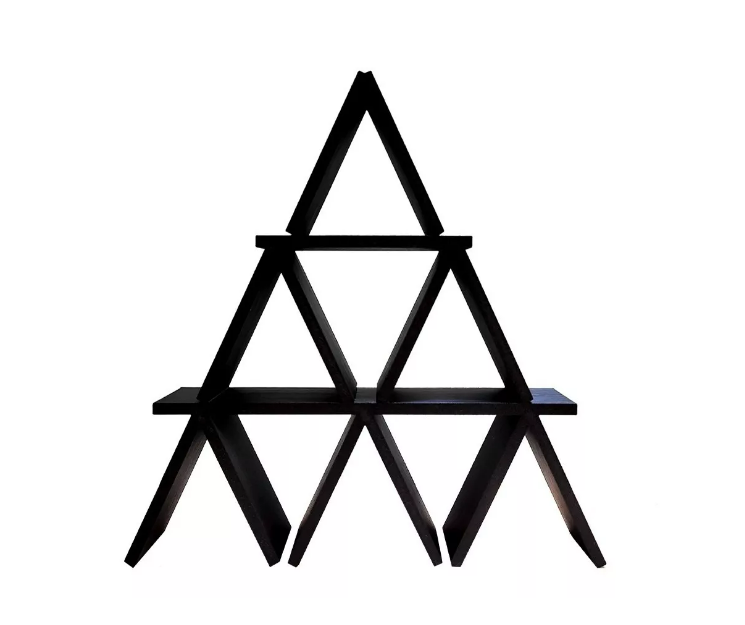
\includegraphics[scale=0.4]{lampada/piramide.png}
\end{center}

\subsection*{Entrada}
A entrada possui somente uma linha e contém a altura $h$ ($1 \leq h \leq 10^9$) da pirâmide que Aladdin precisa montar.

\subsection*{Saída}
Imprima 1 linha com a quantidade de cartas necessárias para montar uma pirâmide de altura $h$.

\begin{table}[!h]
\centering
\begin{tabular}{|l|l|}
\hline
\begin{minipage}[t]{3in}
\textbf{Exemplo de entrada}
\begin{verbatim}
1
\end{verbatim}
\vspace{1mm}
\end{minipage}
&
\begin{minipage}[t]{3in}
\textbf{Exemplo de saída}
\begin{verbatim}
2
\end{verbatim}
\vspace{1mm}
\end{minipage} \\
\hline
\end{tabular}
\end{table}
\begin{table}[!h]
\centering
\begin{tabular}{|l|l|}
\hline
\begin{minipage}[t]{3in}
\textbf{Exemplo de entrada}
\begin{verbatim}
10
\end{verbatim}
\vspace{1mm}
\end{minipage}
&
\begin{minipage}[t]{3in}
\textbf{Exemplo de saída}
\begin{verbatim}
155
\end{verbatim}
\vspace{1mm}
\end{minipage} \\
\hline
\end{tabular}
\end{table}


\end{document}
